\documentclass[aspectratio=169]{beamer}
\newcommand{\sourcepath}[1]{../#1}
%\newcommand{\stylepath}[1]{../beamer/#1}


\usepackage{\sourcepath{beamer/beamerthemeLCS27}}
%\usepackage{indentfirst}

\background{../fig/BeihangPicture.jpg}
\schoollogo{../fig/BeihangLogo.jpg}
%\lablogo{../fig/CentraleSupelecRVB.jpg}

\title{一个\LaTeX模板}
\author{LCS27}

\institute{My dear institute}
\date{\today}



\begin{document}

\maketitle
\begin{frame}{目录}
\tableofcontents
\end{frame}
\section{章节一}
\begin{frame}{标题一}{简述}
\zhlipsum[10]
\end{frame}

\section{章节二}
\begin{frame}[allowframebreaks]{标题二}{简述}
\zhlipsum[11]
\end{frame}
\begin{frame}[allowframebreaks]{标题三}{简述}
\zhlipsum[12]
\end{frame}

\section{章节三}
\subsection{副章节一}
\begin{frame}[allowframebreaks]{标题四}{具体内容}
\zhlipsum[1]
\begin{figure}
    \centering
    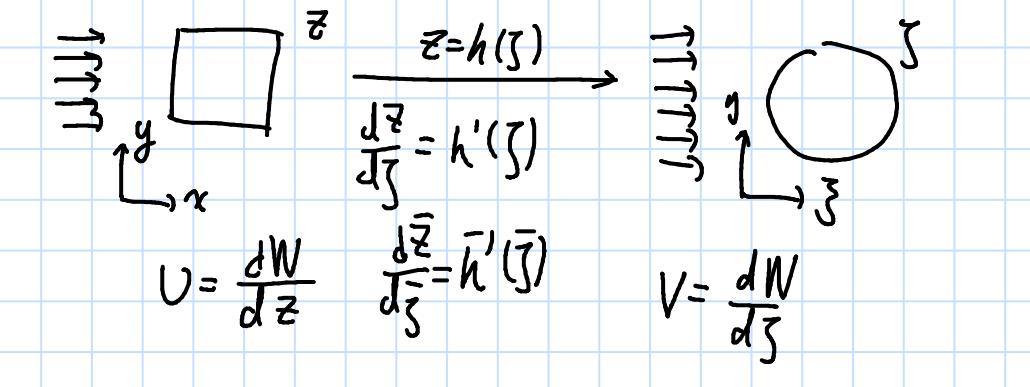
\includegraphics[width=0.5\textwidth]{../picture/1.jpg}
\end{figure}
\end{frame}
\subsection{副章节二}
\begin{frame}[allowframebreaks]{标题五}{具体内容}
\zhlipsum[2]
\begin{itemize}
    \item \zhlipsum[3]
    \item \zhlipsum[4]
    \item \zhlipsum[5]
\end{itemize}
\end{frame}

\begin{frame}{标题六}{具体内容}
\begin{block}{block title}
ABCDSGJGAJLHKL8
\end{block}
\end{frame}
\end{document}
